\chapter{Architecture}

\section{Architecture système}

\begin{figure}[H]
    \centering
    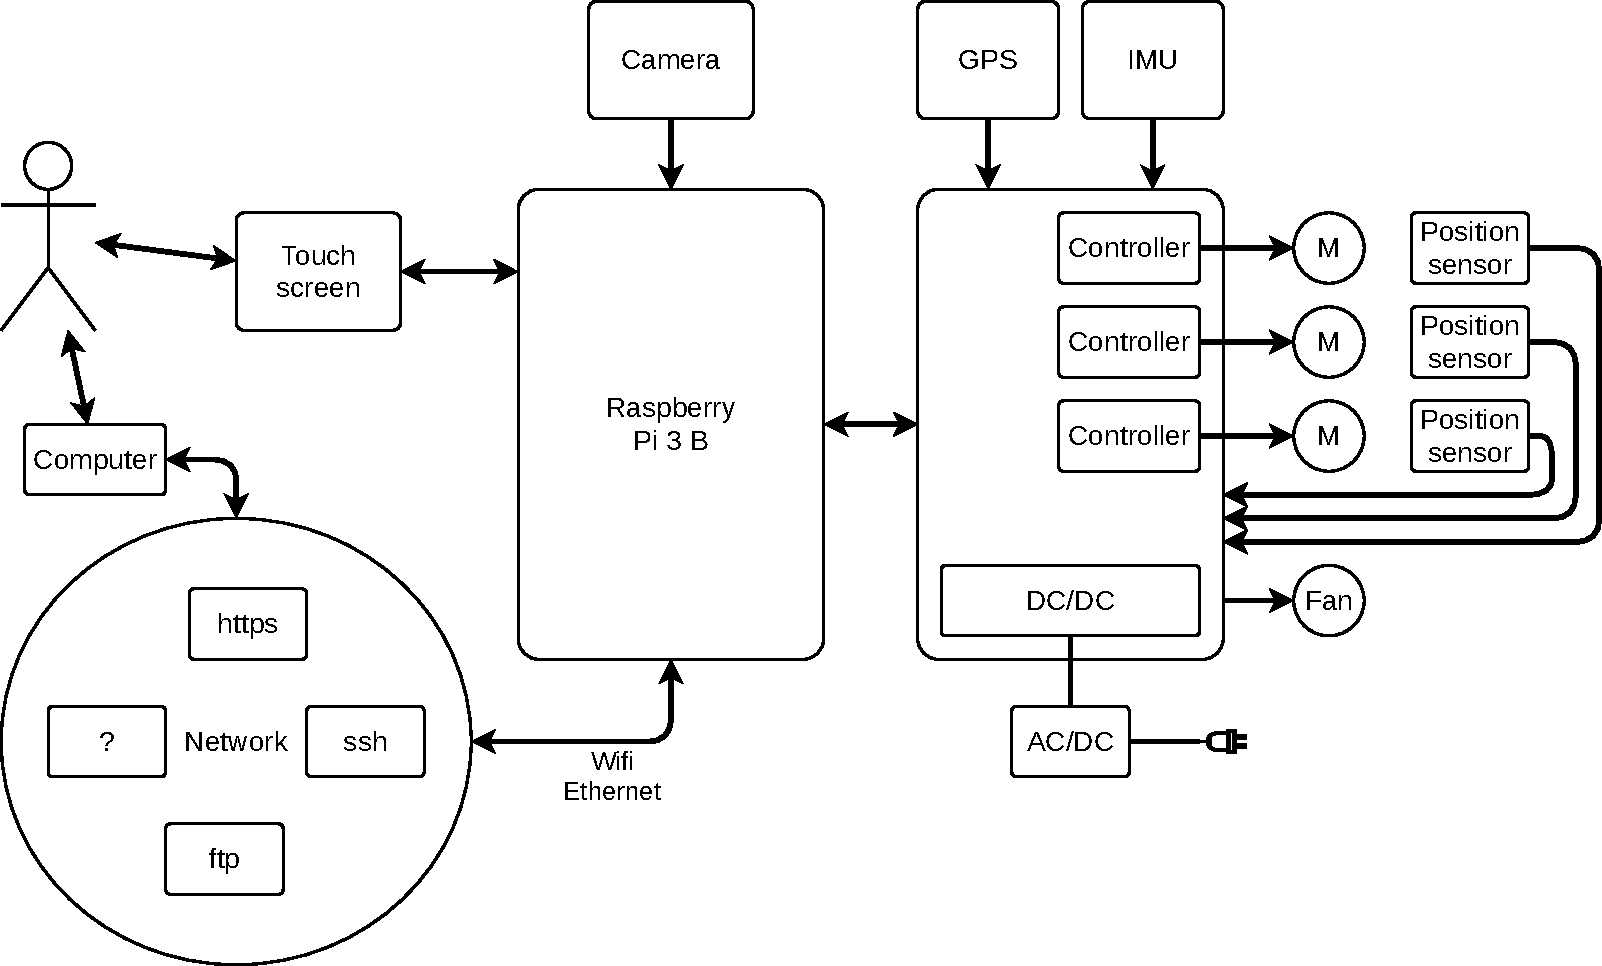
\includegraphics[width=1\linewidth]{\figures/sch_functionnal.pdf}
    \decoRule
    \caption[
    Schéma fonctionnel du télescope]{
    Schéma fonctionnel du télescope}
    \label{fig:Schéma fonctionnel du télescope}
    \end{figure}

\vspace{1cm}

Le télescope sera composé d'une carte Raspberry Pi à laquelle sera connecté une carte de même format accueillant le module GPS, le module IMU (centrale inertielle), les contrôleurs des moteurs ainsi que l'alimentation du système. Les modules GPS et IMU seront probablement déportés afin de les éloigner des moteurs et de leurs perturbations électromagnétiques.

La caméra et l'éventuel écran tactile seront directement connectés à la Raspberry Pi.

Trois moteurs permettront de mouvoir le télescope~:
\begin{itemize}[label=$\bullet$]
	\item Un pour l'azimut.
	\item Un pour l'élévation.
	\item Un pour le zoom.
	\end{itemize}

\vspace{1cm}

Pour interagir avec le télescope, l'utilisateur aura le choix d'utiliser l'éventuel écran tactile embarqué ou bien un ordinateur connecté au télescope via le réseau. Cette solution étant la voie d'accès préférentielle aux contrôles du télescope.

\section{Architecture logicielle}

\begin{figure}[H]
    \centering
    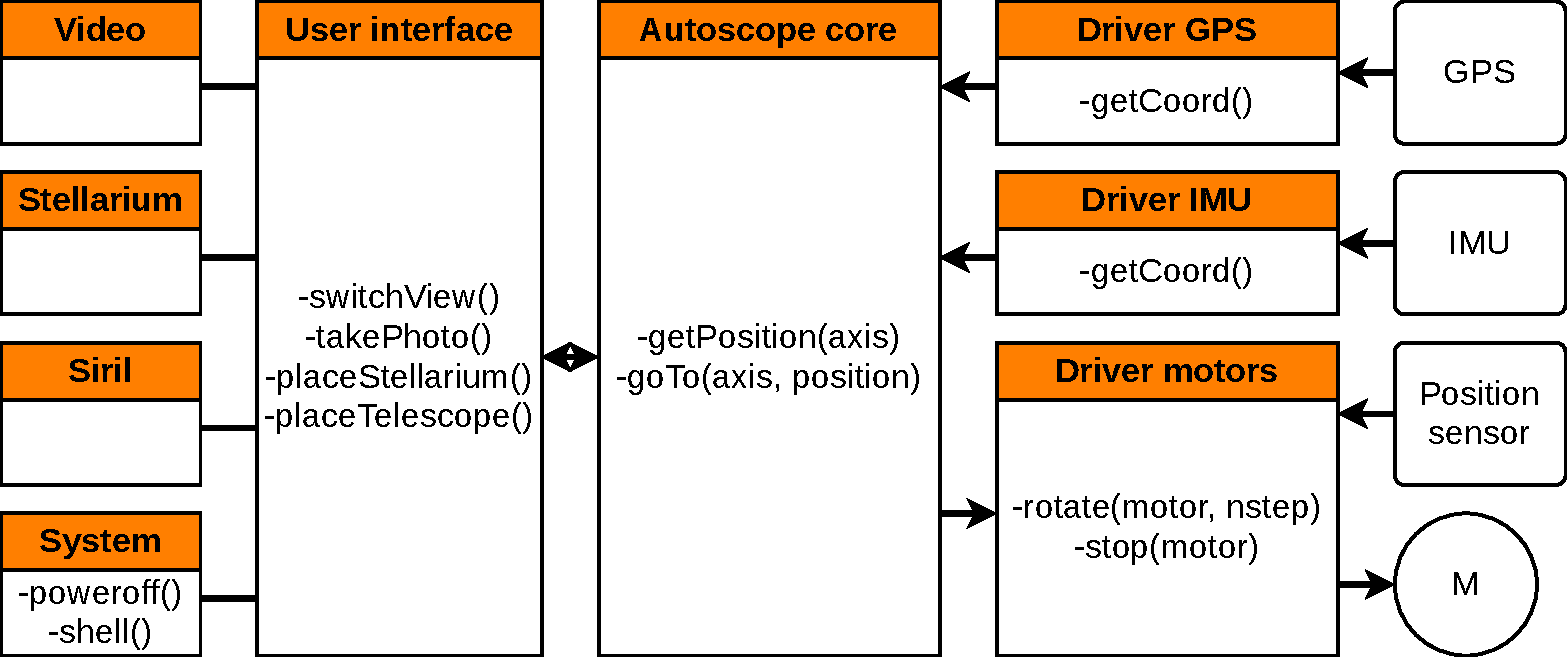
\includegraphics[width=0.9\linewidth]{\figures/sch_software.pdf}
    \decoRule
    \caption[
    Architecture logicielle du télescope]{
    Architecture logicielle du télescope}
    \label{fig:Architecture logicielle du télescope}
    \end{figure}

\vspace{1cm}

Le fonctionnement du télescope reposera sur plusieurs briques logicielles.
\begin{itemize}[label=$\bullet$]
	\item Au plus bas niveau les drivers élémentaires permettant de recueillir les données que fournissent l'IMU et le GPS, ainsi que d'actionner les moteurs, ceux-ci étant asservis par des capteurs de positions extrêmes.
	\item À l'étage suivant le logiciel principal du télescope permettant de connaître les coordonnées précises du télescope (position géographique, orientation spatiale) et d'ordonner au télescope d'adopter une orientation particulière.
	\item À l'étage supérieur l'interface utilisateur permettant de prendre des clichés du ciel, d'orienter le télescope selon Stellarium, de placer Stellarium selon l'orientation du télescope, mais avant tout de basculer entre les différents modes du télescope~:
	\begin{itemize}
		\item Observation du ciel via la caméra.
		\item Exploration virtuelle du ciel avec Stellarium (local ou distant).
		\item Amélioration d'images avec Siril.
		\item Interaction avec le système d'exploitation du télescope.
		\end{itemize}
	\end{itemize}


